
\chapter{Exploratory Data Analysis: univariate}
\label{ch:edaUnivariate}

\index{Exploratory Data Analysis (EDA)}

The fancy term ``\textbf{Exploratory Data Analysis}'' (EDA) basically just
means getting acquainted with your data. After importing a new data set into
Python, the first thing you normally do is poke around to get an idea of what
it contains. You may not even know what questions you eventually want to ask --
let alone what the answers are -- but sizing up the data is a necessary
precursor to those activities.

\index{univariate}

In this chapter, we'll learn some basic EDA techniques for \textbf{univariate
data}, which is really all we've studied so far. ``Univariate'' means to
consider just one variable at a time, rather than possible relationships
between variables. A single (one-dimensional) NumPy array or Pandas
\texttt{Series} is a univariate data set, if you treat it in isolation. As it
turns out, there's quite a few interesting things you can do with even
something that simple.

\index{summary statistics}

\index{scales of measure}
\index{categorical variable}
\index{nominal variable}

First, we'll look at \textbf{summary statistics}, which are a way to capture
the general features of a data set so you can see the forest instead of just a
bunch of trees. Which type of summary information is appropriate depends on
whether you're dealing with categorical or numeric data.

\section{Categorical data: counts of occurrences}

\label{categoricalDataValueCounts}

\index{faves@\texttt{faves}}
\index{Swift@Taylor Swift}
\index{Perry@Katy Perry}

Let's say you had access to a poll on people's favorite pop stars. You import
this into a big ol' Pandas \texttt{Series} called \texttt{faves}:

\begin{Verbatim}[fontsize=\scriptsize,samepage=true,frame=single,framesep=3mm]
print(faves)
\end{Verbatim}

\begin{Verbatim}[fontsize=\scriptsize,samepage=true,frame=leftline,framesep=5mm,framerule=1mm]
0          Katy Perry
1             Rihanna
2       Justin Bieber
3               Drake
4             Rihanna
5        Taylor Swift
6               Adele
7               Adele
8        Taylor Swift
9       Justin Bieber
...
1395       Katy Perry
dtype: object
\end{Verbatim}

\index{value\_counts@\texttt{.value\_counts()} method (Pandas)}

That's great, but it's also kinda TMI. You probably don't care who the
\textit{first} person's idol is, nor the fifteenth, nor the last. Much more
interesting is simply \textit{how many times} each value appears in the
\texttt{Series}. This information is available from the Pandas
\texttt{.value\_counts()} method:

\begin{Verbatim}[fontsize=\small,samepage=true,frame=single,framesep=3mm]
counts = faves.value_counts()
print(counts)
\end{Verbatim}

\begin{Verbatim}[fontsize=\small,samepage=true,frame=leftline,framesep=5mm,framerule=1mm]
Taylor Swift     388
Katy Perry       265
Drake            261
Adele            212
Rihanna          136
Justin Bieber    134
dtype: int64
\end{Verbatim}

The \texttt{.value\_counts()} method returns another \texttt{Series}, but the
\textit{values} of the original \texttt{Series} become the \textit{keys} of the
new one. This tells us at a glance how popular each answer is relative to the
others.

To get percentages instead of totals, just divide by the total and multiply by
100, of course:

\begin{Verbatim}[fontsize=\small,samepage=true,frame=single,framesep=3mm]
print(counts / len(counts) * 100)
\end{Verbatim}

\begin{Verbatim}[fontsize=\small,samepage=true,frame=leftline,framesep=5mm,framerule=1mm]
Taylor Swift     0.277937
Katy Perry       0.189828
Drake            0.186963
Adele            0.151862
Rihanna          0.097421
Justin Bieber    0.095989
dtype: float64
\end{Verbatim}

\index{mode}
\index{central tendency}
\index{measure of central tendency}

Recall (p.~\pageref{mode}) that the \textbf{mode} is the only measure of
central tendency that makes sense for categorical data. And all you have to do
is call \texttt{.value\_counts()} and look at the top result. (In this case,
\texttt{Taylor Swift}.)

Note that \texttt{.value\_counts()} is a Pandas \texttt{Series} method, not a
NumPy method. If you find yourself with a NumPy array instead, you can just
\textbf{wrap} it in a \texttt{Series} as we did in Section~\ref{wrap}
(p.~\pageref{wrap}):

\begin{Verbatim}[fontsize=\small,samepage=true,frame=single,framesep=3mm]
my_array = np.array(['red','blue','red','green','green','green','blue'])
print(pd.Series(my_array).value_counts())
\end{Verbatim}

\begin{Verbatim}[fontsize=\small,samepage=true,frame=leftline,framesep=5mm,framerule=1mm]
green    3
red      2
blue     2
dtype: int64
\end{Verbatim}

\section{Numerical data: quantiles}

\label{quantiles}
\index{real number}
\index{quantile}
\index{cut point (quantile)}

A \textbf{quantile} is a real number between 0 and 1 that represents a
``\textbf{cut point}'' of a numerical data set: roughly speaking, it's the
number for which a certain fraction of the values are \textit{less than} that
number. So the ``.2-quantile'' (pronounced ``point two quantile'') of a
variable containing the heights of third-graders might be 50 inches. If that's
the case, it would indicate that \textit{20\% of the third-graders are less
than 50 inches tall.}

Quantiles are very revealing, but underappreciated. Most people don't seem to
know how to interpret them. But once you figure it out, you'll realize that
quantiles tell you almost everything possible to know about a numeric variable:
by dialing the quantile between 0 and 1, you can tell exactly how common values
in a certain range are.

\index{quantile@\texttt{.quantile()} method (Pandas)}

In Python, you simply call the \texttt{.quantile()} method on a
\texttt{Series}, passing a number between 0 and 1 as an argument, and it tells
you exactly where that cut point is.

Now there's a little bit of weirdness around the edges, depending on the exact
definition used to calculate the quantiles. Let's say I collected some salary
data, and got these responses (``k'' means ``thousand dollars per year,'' and
``M'' means ``million dollars per year''):

\begin{center}
35k\quad 22k\quad 67k\quad 45k\quad 35k\quad 8M\quad 94k\quad 51k\quad 53k\quad
64k\quad 54k
\end{center}

How would I calculate, say, the .7-quantile? First, sort the numbers:

\begin{center}
22k\quad 35k\quad 35k\quad 45k\quad 51k\quad 53k\quad 54k\quad 64k\quad 67k\quad 94k\quad 8M
\end{center}

(yes, we \textit{do} include the 35k value twice; don't eliminate duplicates)
and then spread out the quantiles ``evenly'' from 0 to 1:

\begin{center}
\renewcommand{\arraystretch}{.7}
\begin{tabular}{rccccccccccc}
value: & 22k& 35k& 35k& 45k& 51k& 53k& 54k& 64k& 67k& 94k& 8M\\
& $\uparrow$ &
$\uparrow$ &
$\uparrow$ &
$\uparrow$ &
$\uparrow$ &
$\uparrow$ &
$\uparrow$ &
$\uparrow$ &
$\uparrow$ &
$\uparrow$ &
$\uparrow$ \\
quantile: & .0\ \ & .1\ \  & .2\ \  & .3\ \  & .4\ \  & .5\ \  & .6\ \  & .7\ \  & .8\ \  & .9\ \  & 1.0 \\
\end{tabular}
\end{center}

Don't get picky on me. If you were picky, you could quibble at saying ``the
.3-quantile is 45k'' since it's technically \textit{not} true that 30\% of the
values are less than 45k: in truth, 3 out of 11 (27.3\%) of them are. Whatever,
whatever. The point is that 45k is at the ``cut point'' that's
$\frac{3}{10}$ths of the way through the values from min to max. Quantiles
aren't about laser precision anyway: they're about understanding the general
pattern of the data.

\subsection{``Special'' quantiles}

\index{median}

You'll realize as an immediate consequence of the above that the
\textbf{median} is just another name for the \textbf{.5-quantile}. It's the
value for which half the data points are below it, and half above. Also, the
\textbf{0-quantile} is just the minimum of the data set, and the
\textbf{1-quantile} the maximum.

\subsection{Other kinds of ``-tiles''}

This whole idea may ring bells with other names for you: qua\textbf{r}tiles,
qu\textbf{i}ntiles, deciles, or (most probably) percentiles. All of those are
basically special cases of quantiles. They split the data into evenly-sized
groups:

\index{quartile}
\index{quintile}
\index{quantile}
\index{decile}
\index{percentile}

\begin{compactitem}
\item ``quartiles'': split the data into four groups, with the split points
being the .25-, .5-, and .75-quantiles.
\item ``quintiles'': split the data into five groups, with the split points
being the .2-, .4-, .6, and .8-quantiles.
\item ``deciles'': split the data into ten groups, with the split points
being the .1-, .2-, .3-, .4-, .5-, .6-, .7-, .8-, and .9-quantiles.
\item ``percentiles'': split the data into 100 groups, with the split points
being the .01-, .02-, .03-, ..., .98-, and .99-quantiles.
\end{compactitem}

Be careful to understand that ``evenly-sized groups'' does not mean ``groups
with the same-sized range,'' but rather ``groups with \textit{the same number
of data points in them.}'' Normally, in fact, the ranges will \textit{not} be
the same size. The lowest quintile for a data set of IQs might range from 47
(the lowest IQ in the data set) all the way up to 83, whereas the IQs in the
middle quintile might all be in the narrow range 96 to 104.

\subsection{A quantile example}

\index{YouTube}
\index{num\_plays@\texttt{num\_plays}}

Let's nail this down with an example. I have a (fictitious) data set containing
the number of YouTube plays for each of a selection of videos. It's called
\texttt{num\_plays}. Here are the first few values:

\begin{Verbatim}[fontsize=\small,samepage=true,frame=leftline,framesep=5mm,framerule=1mm]
0     791
1    3133
2       0
3    1789
4     297
5     219
6    1688
7     209
8     422
9   91454
dtype: int64
\end{Verbatim}

That's great, but it's both too much information and too little: we can pore
through the plays for every single video, but it's hard to get our head around
what the overall contents are. So let's run some quantiles. We'll start with
the .1-quantile:

\begin{Verbatim}[fontsize=\small,samepage=true,frame=single,framesep=3mm]
print(num_plays.quantile(.1))
\end{Verbatim}
\vspace{-.3in}

\begin{Verbatim}[fontsize=\small,samepage=true,frame=leftline,framesep=5mm,framerule=1mm]
0.0
\end{Verbatim}

\label{pointOneQuantileEpiphany}
Whoa. The .1-quantile is \textit{zero}. Think about what that means.
Pictorially, sorting the data would give this:

\begin{center}
\renewcommand{\arraystretch}{.7}
\begin{tabular}{rccccccccccccc}
value: & 0& 0& 0& 0& 0& 0& 0& 0& $\cdots$ & 0 & 0 & $\cdots$ \\
& $\uparrow$ & & & & & & & & & & $\uparrow$ & \\
quantile: & .0\ \ & & & & & & & & & & .1\ \ & \\
\end{tabular}
\end{center}

Put another way, that means that (at least) \textit{10\% of our videos have no
plays at all.}

Let's try the .2-quantile:

\begin{Verbatim}[fontsize=\small,samepage=true,frame=single,framesep=3mm]
print(num_plays.quantile(.2))
\end{Verbatim}
\vspace{-.3in}

\begin{Verbatim}[fontsize=\small,samepage=true,frame=leftline,framesep=5mm,framerule=1mm]
15.0
\end{Verbatim}

Okay, now at least we have a pulse. But in case we thought this was data set
was packed with big hits, think again: a full 20\% of these videos have fewer
than 15 plays.

The median is:

\begin{Verbatim}[fontsize=\small,samepage=true,frame=single,framesep=3mm]
print(num_plays.quantile(.5))
\end{Verbatim}
\vspace{-.3in}

\begin{Verbatim}[fontsize=\small,samepage=true,frame=leftline,framesep=5mm,framerule=1mm]
263.0
\end{Verbatim}

That's quite a bit higher. How about the 90\% mark?

\begin{Verbatim}[fontsize=\small,samepage=true,frame=single,framesep=3mm]
print(num_plays.quantile(.9))
\end{Verbatim}
\vspace{-.3in}

\begin{Verbatim}[fontsize=\small,samepage=true,frame=leftline,framesep=5mm,framerule=1mm]
1378.0
\end{Verbatim}

All right, so the upper end of these videos are in the thousands. Finally,
let's look at the max:

\begin{Verbatim}[fontsize=\small,samepage=true,frame=single,framesep=3mm]
print(num_plays.quantile(1))
\end{Verbatim}
\vspace{-.3in}

\begin{Verbatim}[fontsize=\small,samepage=true,frame=leftline,framesep=5mm,framerule=1mm]
982221.0
\end{Verbatim}

!!

Believe it or not, this sort of thing isn't unusual, especially with data from
social phenomena. The tiny fraction of the data at the upper end of the range
is \textit{vastly} higher than everything else is. Get your head around that:
the median number of plays was a couple hundred, but the maximum number of
plays was nearly a \textit{million}.

\section{Numerical data: other summary statistics}

\index{mean}
\index{mean@\texttt{.mean()} method (Pandas)}

That YouTube data set is a good segue to talking about that most overused of
all statistics: the \textbf{mean}. Nearly everyone, if you ask them ``what's
the typical number of plays for these videos?'' will use the mean, or average,
to get at the answer. After all, isn't that what we mean by ``the average
number of plays?''

The answer is: not really, and not usually. Look what happens if we compute the
mean (using the \texttt{.mean()} \texttt{Series} method) in this case:

\begin{Verbatim}[fontsize=\small,samepage=true,frame=single,framesep=3mm]
print(num_plays.mean())
\end{Verbatim}
\vspace{-.3in}

\begin{Verbatim}[fontsize=\small,samepage=true,frame=leftline,framesep=5mm,framerule=1mm]
14018.888235294118
\end{Verbatim}

Consider just how misleading that really is. The ``average'' number of plays is
over 14,000. Yet the \textit{.9}-quantile was less than $\frac{1}{10}$th of that!
In fact, even the .97-quantile is only:

\begin{Verbatim}[fontsize=\small,samepage=true,frame=single,framesep=3mm]
print(num_plays.quantile(.97))
\end{Verbatim}
\vspace{-.3in}

\begin{Verbatim}[fontsize=\small,samepage=true,frame=leftline,framesep=5mm,framerule=1mm]
3836.0
\end{Verbatim}

So \textit{over 97\% of the videos have less than the mean of 14,000 plays.} I
think you'll agree that it is nonsensical to claim that ``the typical number of
plays is 14,018,'' no matter how you slice it.

\index{bell-curvy@``bell-curvy''}

We'll see in the next section why the mean is hopelessly skewed here.
Basically, unless the data is symmetrical and ``bell-curvy,'' it gives a
meaningless number. It is almost \textit{always} safer and more illuminating to
look at the median (or other quantiles).

\index{standard deviation}
\index{std@\texttt{.std()} method (Pandas)}

For completeness, one other commonly cited summary statistic is the
\textbf{standard deviation}, which can be computed with the \texttt{.std()}
method:

\begin{Verbatim}[fontsize=\small,samepage=true,frame=single,framesep=3mm]
print(num_plays.std())
\end{Verbatim}
\vspace{-.3in}

\begin{Verbatim}[fontsize=\small,samepage=true,frame=leftline,framesep=5mm,framerule=1mm]
93031.835
\end{Verbatim}

\index{bell-curvy@``bell-curvy''}
The standard deviation is a measure of the ``spread'' of a data set -- a high
number means (in this example) higher variability in the number of plays from
video to video. As with the mean, it's essentially meaningless (no pun
intended) unless the data is nice and bell-curve shaped.

Speaking of which, we'll never be able to judge the ``shape'' of anything
unless we get some graphical plots involved. So let's turn our focus to that.

\section{Plotting univariate data}

\index{univariate}
\label{twoWaysToPlotUnivariateData}

There are basically two useful ways of plotting a \texttt{Series} with
univariate data. In one, you care about the specific labels (\textit{i.e.}
keys, or ``index'') of the values in the \texttt{Series}, and you want them to
be prominent in the plot. In the other, you don't; you just want to show the
values themselves, so you can visualize how they are distributed irrespective
of what label they might have.

Let's do the first one first.

\subsection{Bar charts of labeled data}

\index{CSV@CSV (comma-separated values format)}
\index{extension@extension (filename)}
\index{filename extension}
\index{file!\texttt{.csv}}

Let's read a data set on the world countries with the highest GDP (Gross
Domestic Product). Here's a CSV file called \texttt{gdp.csv}\footnote{Recall
the caveat about filename extensions in the p.~\pageref{extensions} footnote.}:

\begin{Verbatim}[fontsize=\small,samepage=true,frame=single,framesep=3mm]
Nation,Trillions
Italy,2.26
Germany,4.42
Brazil,2.26
United States,21.41
France,3.06
Canada,1.91
Japan,5.36
China,15.54
India,3.16
United Kingdom,3.02
\end{Verbatim}

\index{read\_csv@\texttt{read\_csv()} function (Pandas)}

We'll read that into a \texttt{Series} using our technique from
p.~\pageref{read_csv}:

\begin{Verbatim}[fontsize=\small,samepage=true,frame=single,framesep=3mm]
gdp = pd.read_csv('gdp.csv', squeeze=True, index_col=0, header=None)
print(gdp)
\end{Verbatim}
\vspace{-.3in}

\begin{Verbatim}[fontsize=\small,samepage=true,frame=leftline,framesep=5mm,framerule=1mm]
0
Nation            Trillions
Italy                 2.26
Germany               4.42
Brazil                2.26
United States        21.41
France                3.06
Canada                1.91
Japan                 5.36
China                15.54
India                 3.16
United Kingdom        3.02
Name: 1, dtype: object
\end{Verbatim}

\index{bar chart}
\index{plot@\texttt{.plot()} method (Pandas)}

and now, we can visualize the relative sizes of these economies with the
\texttt{.plot()} method. The \texttt{.plot()} method takes, among other things,
a ``\texttt{kind}'' argument which specifies what kind of plot you want. In
this case, a \textbf{bar chart} is the correct thing:

\begin{Verbatim}[fontsize=\small,samepage=true,frame=single,framesep=3mm]
gdp.plot(kind='bar')
\end{Verbatim}

\begin{figure}[ht]
\centering
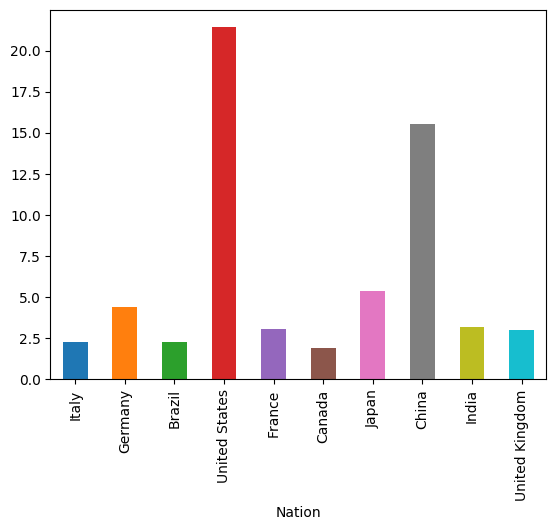
\includegraphics[width=0.7\textwidth]{gdp.png}
\end{figure}

There are a zillion ways to customize these plots, and I'll only mention a
very, very few. A more complete list of options is available by Googling, or
going to \url{https://matplotlib.org/3.1.1/api/\_as\_gen/matplotlib.pyplot.plot.html}

\index{sort\_values@\texttt{.sort\_values()} method (Pandas)}

For instance, to make all the bars the same color, we can pass
``\texttt{color="blue"}''. Sorting the values is something we already know how
to do, with \texttt{.sort\_values()}:

\begin{Verbatim}[fontsize=\small,samepage=true,frame=single,framesep=3mm]
gdp.sort_values(ascending=False).plot(kind='bar')
\end{Verbatim}

\begin{figure}[ht]
\centering
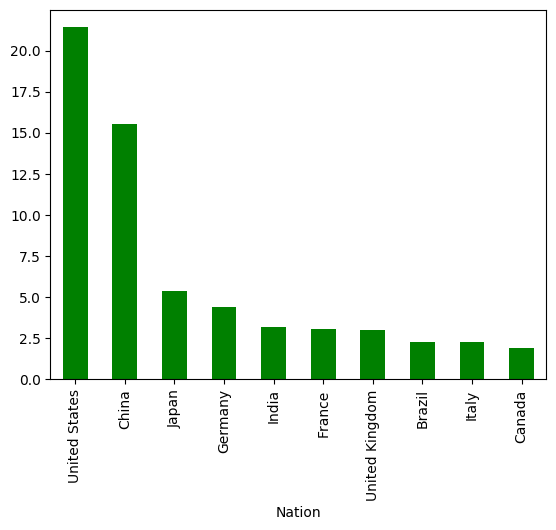
\includegraphics[width=0.7\textwidth]{gdp2.png}
\end{figure}

You see what I mean about ``caring about the labels/keys/index'' for this sort
of plot: if we hadn't labeled the bars, the plot would tell us nothing useful.

I'm sure you've seen lots of bar charts in your life, so this is nothing new.
But consider how much information is embedded in this infographic. Not only can
we tell that the U.S.~and China are the two biggest economies, we can tell that
they are \textit{far and away} the two biggest, with Japan and Germany (the
next two highest) only a fraction.

\subsection{Bar charts of occurrence counts}

\label{categoricalDataBarCharts}

\index{value\_counts@\texttt{.value\_counts()} method (Pandas)}
\index{bar chart}

A very common special case of a bar chart is one where we combine it with the
\texttt{.value\_counts()} method. Let's go back to Taylor vs.~Katy:

\begin{Verbatim}[fontsize=\scriptsize,samepage=true,frame=single,framesep=3mm]
print(faves)
\end{Verbatim}
\vspace{-.3in}

\begin{Verbatim}[fontsize=\scriptsize,samepage=true,frame=leftline,framesep=5mm,framerule=1mm]
0          Katy Perry
1             Rihanna
2       Justin Bieber
3               Drake
4             Rihanna
5        Taylor Swift
6               Adele
7               Adele
8        Taylor Swift
9       Justin Bieber
...
1395       Katy Perry
dtype: object
\end{Verbatim}

\index{plot@\texttt{.plot()} method}

It would be useful to see an infographic on how popular each celebrity is, and
combining \texttt{.value\_counts()} and \texttt{.plot()} makes it a snap:

\begin{Verbatim}[fontsize=\small,samepage=true,frame=single,framesep=3mm]
faves.value_counts().plot(kind='bar',color="orange")
\end{Verbatim}

\begin{figure}[ht]
\centering
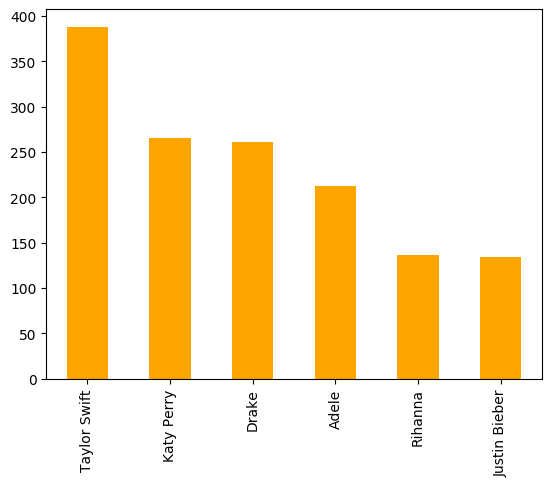
\includegraphics[width=0.6\textwidth]{celebs.png}
\end{figure}

\index{sort\_index@\texttt{.sort\_index()} method (Pandas)}
\index{value\_counts@\texttt{.value\_counts()} method (Pandas)}

The \texttt{.sort\_values()} method wasn't needed here, since
\texttt{.value\_counts()} already returns its answer in decreasing numerical
order. If we wanted the bars in alphabetical order instead, we'd just sort the
\texttt{Series} by index before plotting:

\begin{Verbatim}[fontsize=\small,samepage=true,frame=single,framesep=3mm]
faves.value_counts().sort_index().plot(kind='bar',color="purple")
\end{Verbatim}

\begin{figure}[ht]
\centering
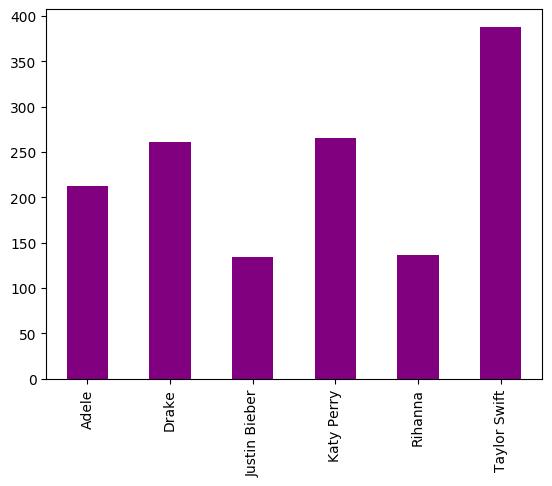
\includegraphics[width=0.6\textwidth]{celebs2.png}
\end{figure}

These long lines with lots of strung-together methods are concise, but can also
be confusing. It's always an option to use temporary variables to store the
intermediate results instead:

\begin{Verbatim}[fontsize=\small,samepage=true,frame=single,framesep=3mm]
counts = faves.value_counts()
alphbetical_counts = counts.sort_index()
alphbetical_counts.plot(kind='bar',color="purple")
\end{Verbatim}

Just a matter of preference.

\section{Numerical data: histograms}

\index{objects (of a study)}

As I mentioned on p.~\pageref{twoWaysToPlotUnivariateData}, sometimes we don't
actually care about the labels in a \texttt{Series}, only the values. This is
when we're trying to size up how \textit{often} values of various magnitudes
appear, irrespective of which specific objects of study those values go with.

\index{histogram}
\index{quantile}
\index{bin (of a histogram)}

My favorite plot this is the \textbf{histogram}. It's super powerful if you
know how to read it, but underused because few people seem to know how. The
idea is that we take a numeric, univariate data set, and divide it up into
\textbf{bins}. Bins are sort of the reverse of quantiles: all bins have the
\textit{same} size range, but a \textit{different} number of data points fall
into each one.

\index{football}
\index{NCAA}

Suppose we had data on the entire history of a particular NCAA football
conference. A \texttt{Series} called ``\texttt{pts}'' has the number of points
scored by each team in all that conference's games. It looks like this:

\begin{Verbatim}[fontsize=\small,samepage=true,frame=single,framesep=3mm]
print(pts)
\end{Verbatim}
\vspace{-.2in}

\begin{Verbatim}[fontsize=\small,samepage=true,frame=leftline,framesep=5mm,framerule=1mm]
0        7
1       35
2       40
3       17
4       10
...
399     14
dtype: int64
\end{Verbatim}

Some basic summary statistics of interest include:

\begin{Verbatim}[fontsize=\small,samepage=true,frame=single,framesep=3mm]
print("min: {}".format(pts.quantile(0)))
print(".25-quantile: {}".format(pts.quantile(.25)))
print(".5-quantile: {}".format(pts.quantile(.5)))
print(".75-quantile: {}".format(pts.quantile(.75)))
print("max: {}".format(pts.quantile(1)))
print("mean: {}".format(pts.mean()))
\end{Verbatim}
\vspace{-.2in}

\begin{Verbatim}[fontsize=\small,samepage=true,frame=leftline,framesep=5mm,framerule=1mm]
min: 0.0
.25-quantile: 17.0
.5-quantile: 25.0
.75-quantile: 32.0
max: 55.0
mean: 23.755
\end{Verbatim}

Looks like a typical score is in the 20's, with the conference record being a
whopping 55 points in one game.

We can plot a histogram of this \texttt{Series} with this code:

\begin{Verbatim}[fontsize=\small,samepage=true,frame=single,framesep=3mm]
pts.plot(kind='hist')
\end{Verbatim}

The result is in Figure~\ref{fig:ncaa1}. Stare hard at it. Python has divided
up the points into ranges: 0 through 6 points, 7 through 12 points, 13 through
21, \textit{etc.} Each of these ranges is a bin. The height of each blue bar on
the plot is simply the number of games in which a team scored in that range.

\begin{figure}[ht]
\centering
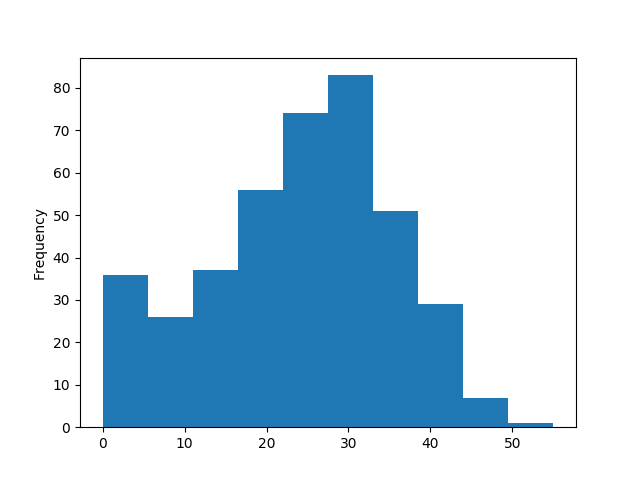
\includegraphics[width=0.9\textwidth]{ncaa1.png}
\caption{A histogram of the historical points-per-game for teams in a certain
NCAA football conference.}
\label{fig:ncaa1}
\end{figure}

\index{bell-curvy@``bell-curvy''}
Now what do we learn from this? Lots, if we know how to read it. For one thing,
it looks like the vast majority of games have teams scoring between 12 and 38
points. A few teams have managed to eke out 40 or more, and there have been a
modest number of single-digit scores or shutouts. Moreover, it appears that
scores between 24 and 38 are considerably more common than those between 12 and
24. Finally, this data shows some evidence of being ``bell-curvy'' in the sense
that values in the middle of the range are more common than values at either
end, and it is (very roughly) symmetrical on both sides of the median.

This is even more precise information than the quantiles gave us. We get an
entire birds-eye view of the data set. Whenever I'm looking at a numerical,
univariate data set, pretty much the first thing I do is throw a histogram up
on the screen and spend at least a couple minutes staring at it. It's almost
the best diagnostic tool available.

\subsection{Bin size}

\index{bin (of a histogram)}
\index{plot@\texttt{.plot()} method (Pandas)}

Now one idiosyncrasy with histograms is that a lot depends on the bin size and
placement. Python made its best guess at a decent bin size here by choosing
ranges of 6 points each. But we can control this by passing a second parameter
to the \texttt{.plot()} function, called ``\texttt{bins}'':

\begin{Verbatim}[fontsize=\small,samepage=true,frame=single,framesep=3mm]
pts.plot(kind='hist', bins=30)
\end{Verbatim}

Here we specifically asked for \textit{thirty} bins in total, and we get the
result in Figure~\ref{fig:ncaa2}. Now each bin is only two points wide, and as
you can see there's a lot more detail in the plot.

\begin{figure}[ht]
\centering
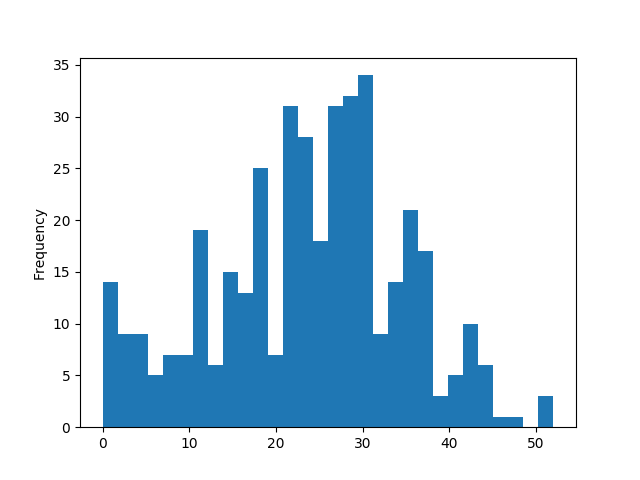
\includegraphics[width=0.9\textwidth]{ncaa2.png}
\caption{The same data set as in Figure~\ref{fig:ncaa1}, but with more (and
smaller) bins.}
\label{fig:ncaa2}
\end{figure}

Whether that amount of detail is a good thing or not takes some practice to
decide. Make your bins too large and you don't get much precision in your
histogram. Make them too small and the trees can overwhelm the forest. In this
case, I'd say that Figure~\ref{fig:ncaa2} is good in that it tells us something
not apparent from Figure~\ref{fig:ncaa1}: there are quite a few shutouts
(zero-point performances), not merely games with six-points-or-less. Whether
the trough between 22 and 24 points is meaningful is another matter, and my
guess is that part is obscuring the more general features apparent in the first
plot.

\index{sweet spot@``sweet spot''}

The rule is: whenever you create a histogram, \textit{take a few minutes to
experiment with different bin sizes.} Often you'll find a ``sweet spot'' where
the amount of detail is just right, and you'll get great insight into the data.
But you do have to work at it a little bit.

\subsection{Non-bell-curvy data}

\index{YouTube}
\index{num\_plays@\texttt{num\_plays}}

Let's return again to the YouTube example. We had some surprises when we looked
at the quantiles and saw that the 1-quantile (max) was astronomically higher
than the .9-quantile was. Let's see what happens when we plot a histogram
(show in Figure~\ref{fig:youtube1}):

\begin{Verbatim}[fontsize=\scriptsize,samepage=true,frame=single,framesep=3mm]
num_plays.plot(kind='hist', color="red")
\end{Verbatim}

\begin{figure}[ht]
\centering
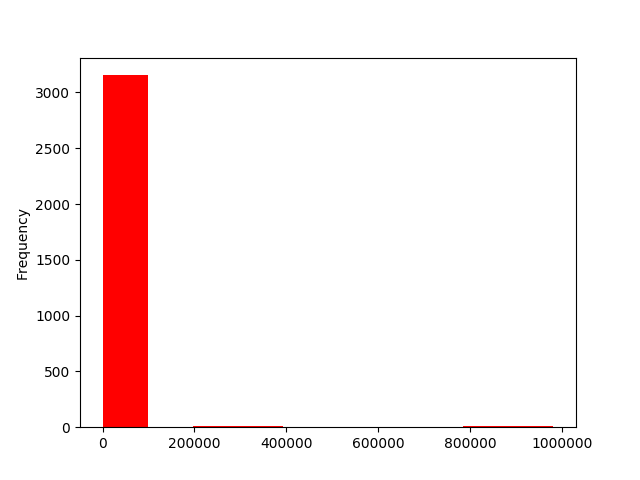
\includegraphics[width=1\textwidth]{youtube1.png}
\caption{A first attempt at plotting the YouTube \texttt{num\_plays} data set.}
\label{fig:youtube1}
\end{figure}

Huh?? Wait, where are all the bars of varying heights? We seem to have got only
a single one.

But they're there! They're just so small you can't see them. If you stare at
the x-axis -- and your eyesight is good -- you might see tiny signs of life at
higher values. But the overall picture is clear: the vast, vast majority of
videos in this set have between 0 and 100,000 plays.

\index{bin (of a histogram)}

Let's see if we can get more detail by increasing the number of bins (say,
to 1000):

\begin{Verbatim}[fontsize=\scriptsize,samepage=true,frame=single,framesep=3mm]
num_plays.plot(kind='hist', bins=1000, color="red")
\end{Verbatim}

We now get the left-hand side of Figure~\ref{fig:youtube23}. It didn't really
help much. Turns out the masses aren't merely crammed below a hundred thousand
plays; they're crammed below \textit{one} thousand. We need another approach if
we're going to see any detail on the low-play videos.

\begin{figure}[ht]
\centering
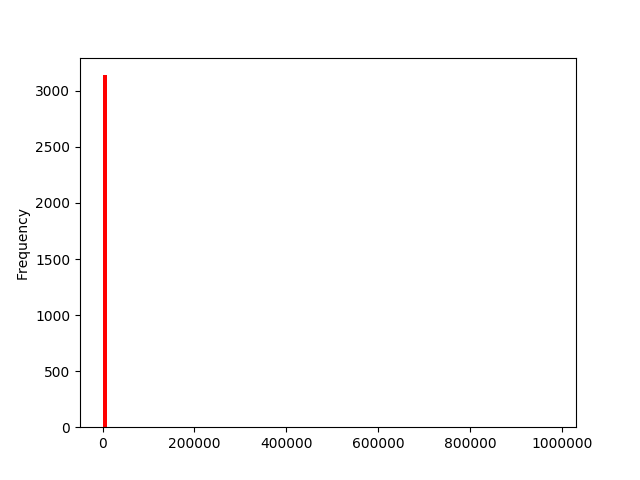
\includegraphics[width=.48\textwidth]{youtube2.png}
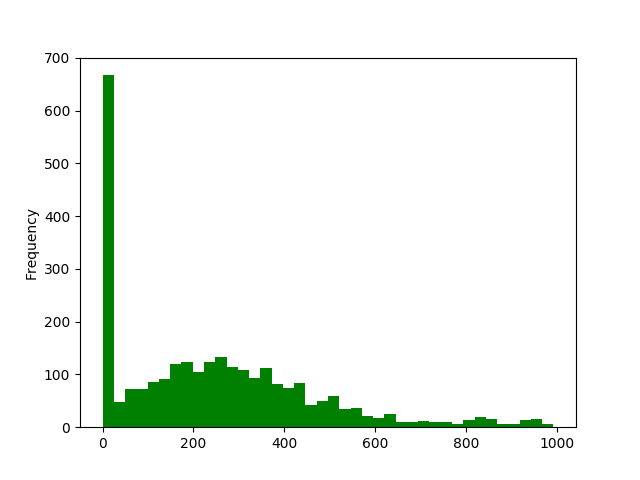
\includegraphics[width=.48\textwidth]{youtube3.png}
\caption{Further attempts at plotting the YouTube \texttt{num\_plays} data set.
On the left side, we decreased the bin size to no avail. On the right side, we
gave up on plotting the popular videos and concentrated only on the unpopular
ones, which does illuminate the lower end somewhat. (Don't miss the x-axis
ranges!)}
\label{fig:youtube23}
\end{figure}


\index{distribution}
\index{query}
\index{filter}

The only way to really see the distribution on the low end is to \textit{only}
plot the low end. Let's use a query (recall section~\ref{seriesQueries} from
p.~\pageref{seriesQueries}) to filter out \textit{only} the videos with 1000
plays or fewer, and then plot a histogram of that:

\begin{Verbatim}[fontsize=\scriptsize,samepage=true,frame=single,framesep=3mm]
unpopular_video_plays = num_plays[num_plays <= 1000]
unpopular_video_plays.plot(kind='hist', color="green")
\end{Verbatim}

This gives the right-hand side of Figure~\ref{fig:youtube23}. Now we can at
least see what's going on. Looks like our \texttt{Series} has a crap-ton of
videos that have never been viewed at all (recall our .1-quantile epiphany for
this data set on p.\pageref{pointOneQuantileEpiphany}) plus a chunk that are in
the 500-views-or-fewer range.

\index{bell-curvy@``bell-curvy''}
\index{mean}
\index{standard deviation}
\index{Broadway shows}

The takeaway here is that not all data sets (by a long shot!) are bell-curvy.
Statistics courses often present nice, symmetric data sets on physical
phenomena like bridge lengths or actor heights or free throw percentages, which
have nice bell curves and are nicely summarized by means and standard
deviations. But for many social phenomena (like salaries, numbers of
likes/followers/plays, lengths of Broadway show runs, \textit{etc.})~the data
looks more like this YouTube example. A few extremely large values dominate
everything else by their sheer magnitude, which makes it more difficult to wrap
your head around.

It also makes it more challenging to answer the question, ``what's the
\textit{typical} value for this variable?'' It ain't the mean, that's for sure.
If you asked me for the ``typical'' number of plays of one of these YouTube
videos, I'd probably say ``zero'' since that's an extremely common value.
Another reasonable answer would be ``somewhere in the low hundreds,'' since
there are quite a few videos in that range, as illustrated by the
right-hand-side of Figure~\ref{fig:youtube23}. But you'd be hard-pressed to try
and sum up the entire data set with a single typical value. There just isn't
one for stuff like this.

\section{Numerical data: box plots}

\index{bivariate}
\index{box plot}
\index{plot@\texttt{.plot()} method (Pandas)}

Let's talk about one more type of plot in this chapter, even though it's really
most useful when dealing with bivariate data, as we'll address in a later
chapter. It's called the \textbf{box plot} (also known as a
``\textbf{box-and-whisker'' plot}). We can create one by passing
``\texttt{kind="box"}'' to the \texttt{.plot()} method (here for the NCAA
football data):

\begin{Verbatim}[fontsize=\small,samepage=true,frame=single,framesep=3mm]
pts.plot(kind="box")
\end{Verbatim}

The result is shown in Figure~\ref{fig:ncaaBox}, along with some annotations in
red so you can figure out what's going on.

\begin{figure}[ht]
\centering
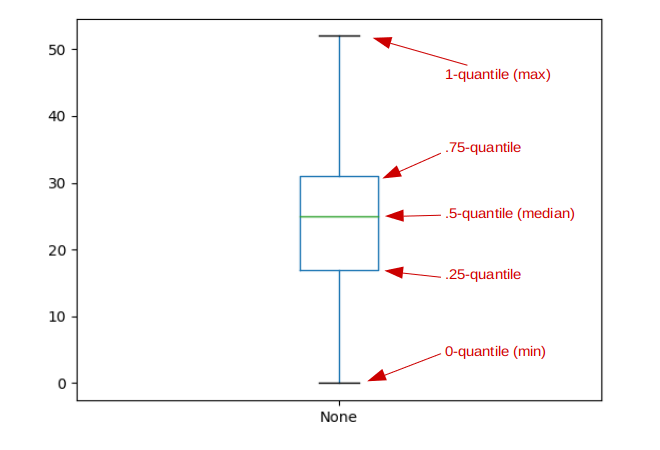
\includegraphics[width=1\textwidth]{ncaaboxAnnotated.png}
\caption{A box plot of the NCAA points data.}
\label{fig:ncaaBox}
\end{figure}

For now, don't worry about the mysterious word ``\texttt{None}'' at the bottom.
(This indicates which ``group'' the box represents, and will feature
prominently in our bivariate data chapter.) For a univariate data set like this
one, the x-axis has no meaning. The y-axis, on the other hand, is easy to
understand: it's the number of points per football game.

\index{quantile}

Now the thing to realize about box plots is that they're essentially just a
graphical way of showing quartiles; or, put another way, a graphical way of
showing these five quantiles:

\begin{compactitem}
\item The 0-quantile (the minimum value) is the y-value of the bottom ``whisker.''
\item The .25-quantile is the y-value of the bottom of the ``box.''
\item The .5-quantile (the median) is the y-value of the horizontal line within
the box.
\item The .75-quantile is the y-value of the top of the ``box.''
\item The 1-quantile (the maximum value) is the y-value of the top ``whisker.''
\end{compactitem}

Using your quantile knowledge from section~\ref{quantiles}, you'll realize the
following fact: \textit{the box alone contains exactly half the data points.}
This is a key insight. While the whiskers show the entire range of the data,
the box shows the middle 50\% of it. This makes it very easy to grasp where the
bulk of the data lies, and it reinforces the lesson we learned from the
histogram on this data set (Figure~\ref{fig:ncaa1} on page
\pageref{fig:ncaa1}): a big chunk of the time, teams score in the 20's.

You might object to showing an entire plot for this, since I've just revealed
that it's merely a fancy way to show five numbers. And you're right, in a way.
However, when we show multiple \textit{groups} of data side-by-side, each with
their own box, it becomes a particularly powerful tool. Stay tuned for that.

\subsection{Outliers}

What happens if we show our head-scratching YouTube data set as a box plot? You
get the monstrosity in Figure~\ref{fig:youtubebox}.

\begin{figure}[ht]
\centering
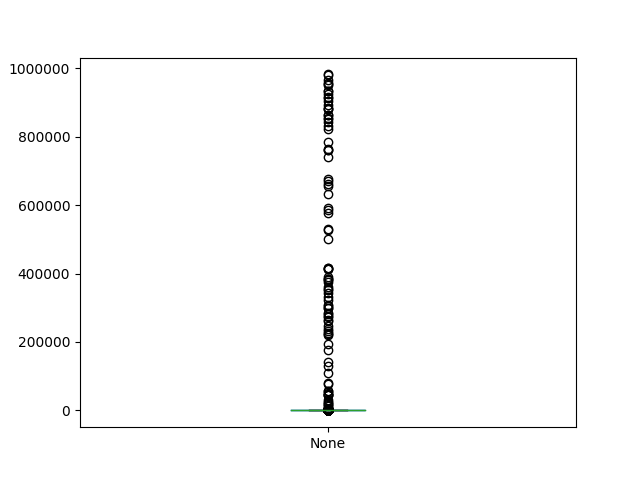
\includegraphics[width=0.8\textwidth]{youtubebox.png}
\caption{A box plot of a non-bell-curvy data set.}
\label{fig:youtubebox}
\end{figure}

\index{outlier}
\index{fish bubbles}

Geez Louise, does that look wacky. The little circles (which to me always
looked like bubbles from fish breath) represent \textbf{outliers}, an important
concept in data science. An outlier is basically any data point that's so far
out of the normal range that it seems strange. Python is essentially flagging
it for us, so we can judge for ourselves whether it was a data entry error or
just a strange data point. In this case, these aren't errors -- there's just a
handful of videos that have been played a ton of times. And this makes the
whole box plot look weird.

\index{gravity}
\index{black hole}
\index{smoosh}

Notice from Figure~\ref{fig:youtubebox} that \textit{the entire box and both
whiskers} have gotten smooshed at the bottom of the figure, as if crushed by
the gravity of a black hole. You'll see that the top whisker doesn't
\textit{really} mean ``maximum,'' since it's way down there in thousand-land
despite the fact that we have videos with almost a million views. The top
whisker truly means ``the maximum \textit{reasonable-looking} data point in the
\texttt{Series},'' where ``reasonable-looking'' is something Pandas is trying
to make an educated guess about. There are ways to tweak what counts as an
outlier, but my purpose here is just to get you to realize that when you have a
highly skewed data set (like YouTube), prepare to see lots of things that are
considered ``outliers,'' and prepare to comb through all the mess on your box
plots to try and discern the true meaning it's trying to convey.
